\section{Complexity of \pbm}
\label{sec:proofs_complexity}


        % \noindent Let $I_b = \{ b \in \rat \mid b = b_{\alpha} \text{ or } b = e_{\alpha}
        % \text{ for every }
    % \alpha \text{ specified in } compac(G) \text{ or  } \alpha \text{ specified in } q \} $

    % Let $\alpha_{1},\dotsc,\alpha_{k}$ be a finite set of intervals, where $\alpha_i$ is either specified in the
    % graph or in the query.



% \propPspaceMemb*
\begin{proof}
    $ $\newline

    \noindent Let $I_{\Omega}$ be the set of rational numbers $\mathrm{b}$ such that $\mathrm{b} = b_{\tau}$ or $b =
    e_{\tau}$ for every interval
    $\tau$ specified in both $compac(G)$ and in $q$. Since $b \in \rat$, so it can be
    specified as a fraction, i.e., $\frac{p}{q}$, where $p,q \in
    \mathbb{Z}$ and $q \neq 0$. We say that
    $\mathrm{denom}(\frac{p}{q})=q$. Then $g$ be the
    granularity of the graph,
    i.e.,
    % \[
    %     g=\prod_{i=1}^k \mathrm{denom}(b_{\alpha_i}) \times \mathrm{denom}(e_{\alpha_i})
    % \]
    \[
        g=\prod_{i=1}^{\lvert I_{\Omega} \rvert} \mathrm{denom}(\mathrm{b})
    \]

    \begin{lemma}\label{lemma:interval_boundaries}
    If $\langle o_1,o_2,\tau,d \rangle$ is a compact answer to $q$, then the denominator of $b_{\tau}$ and
    and the denominator of $e_{\tau}$ divide $g$.

  \end{lemma}
  \begin{proof}

      \emph{Proof sketch}. We know that we navigate temporal dimension of $G$ using only $\tndelta$
      operator. The definition of $\evalcit{\tndelta}$ requires exactly two
      arithmetic operations addition and subtraction. If the denominators of starting interval
      divide $g$, then after applying $\tndelta$, the denominators of ending
      interval also divide $g$.    

  \end{proof}


    % That means that the denominator of each interval boundary specified in the graph and in the query divides $g$.

    
    \noindent Let $K=\{\frac{j}{2g} \mid j \in \mathbb{Z} \}$. Let $l$ be the
    greatest lower bound in $K$ such that $l < b_{\tau}$ and $l = b_{\tau} -
    \frac{1}{2g}$. Similarly, let $m$ be the lowest upper bound in $K$ such that $m >
    e_{\tau}$ and $m = e_{\tau} + \frac{1}{2g}$. \\
    
    \noindent We claim that $\langle o_1,o_2,\tau,d \rangle \in \evalcit{q}$
    iff $\langle
    o_1, l,o_2,l+d \rangle \not\in
    \eval{q}$ and $\langle
    o_1,m,o_2,m+d \rangle \not\in
    \eval{q}$ and for every $k \in K$, if $k \in \tau$, then $\langle o_1, k, o_2, k+d \rangle \in \eval{q}$. \\

    \noindent $(\implies).$ Trivially holds from the definition of $\evalcit{q}$. \\\\
    \noindent $(\impliedby).$ If $\langle
    o_1, l,o_2,l+d \rangle \not\in
    \eval{q}$ and $\langle
    o_1,m,o_2,m+d \rangle \not\in
    \eval{q}$ and for every $k \in K$, if $k \in \tau$, then $\langle o_1, k,
    o_2, k+d \rangle \in \eval{q}$. Then $\langle o_1,o_2,\tau,d \rangle \in
    \evalcit{q}$. \\

    \noindent We prove the above statement by contradiction. 

    % We  assume
    % $\langle
    % o_1, l,o_2,l+d \rangle \not\in
    % \eval{q}$ and $\langle
    % o_1,m,o_2,m+d \rangle \not\in
    % \eval{q}$ and for every $k \in K$, if $k \in \alpha$, then $\langle o_1, k,
    % o_2, k+d \rangle \in \eval{q}$ is true and 


    We assume for every $k \in K$, if $k \in \tau$, then $\langle o_1, k,
    o_2, k+d \rangle \in \eval{q}$. Assume $\langle o_1,o_2,\tau,d
    \rangle \in \evalcit{q}$ is false. For the simplicity, assume $q$ is a
    boolean query. Then $q$ does not continuously
    hold on $\tau$ which implies there is a $t \in \tau$ such that $t \not\in K$ and $q$ does not hold on $t$.
    % $\langle o_1, t,
    % o_2, t+d \rangle \not\in \eval{q}$.
Let $p$ be the predecessor of $t$ and $s$ be the successor of t. Since $p,s
    \in K$, so by our assumption $q$ holds on $p$ and $s$.  
    % $\implies$ $\langle o_1, p,
    % o_2, p+d \rangle \in \eval{q}$ and $\langle o_1, s,
    % o_2, s+d \rangle \in \eval{q}$ from the assumption. \\\\
Then $p$ and $s$ are the boundaries of the intervals where $q$ holds. From the
definition of $K$, the numerator of every $k \in K$ is either even or odd and if the numerator of $k$ 
is odd then, $\mathrm{denom}(k)$ is $2g$. Since $t$ lies
between $p$ and $s$ and $p,s \in K$, so either the numerator of $p$ is odd or
the numerator of $s$ is odd. As shown in Figure. \ref{fig:pspace}, the numerator of $p$
is odd. Since we know that if the numerator of $k \in K$ is odd, then the denominator is $2g$ which does
not divide
$g$, which implies either $p$ does not divide $g$ or $s$ does not divide $g$
but according to our lemma \ref{lemma:interval_boundaries} both $p$ and $s$ must divide $g$ that means either $q$ does not hold on $p$ or $q$ does not hold on $s$ that contradicts with our assumption that $q$ holds on both $p$ and $s$.\\ 


\end{proof}


\begin{figure}[!htbp]
\centering
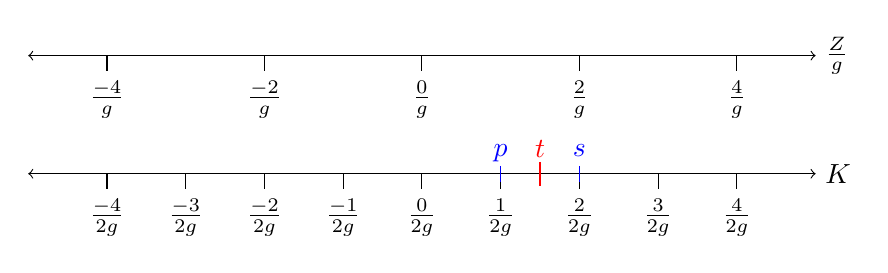
\begin{tikzpicture}

   \draw[<->] (-5,0) -- (5,0) node[right] {$K$};
  \foreach \x in {-4,...,4}
    \draw (\x, 0) -- (\x, -0.2) node[below]{\bfseries
        $\frac{\x}{2g}$};
    % \draw[fill] (1.5,0) circle (0.10) node [yshift=0.6cm, anchor=north]
    %     {$\alpha_2$};
    \draw[red, thick] (1.5,0.15) -- (1.5,-0.15) node [yshift=0.7cm, anchor=north]
        {$t$};
    \draw[blue] (1,0.1) -- (1,-0.1) node [yshift=0.6cm, anchor=north]
        {$p$};
    \draw[blue] (2,0.1) -- (2,-0.1) node [yshift=0.6cm, anchor=north]
        {$s$};

    % first number line
    \draw[<->, yshift=1.5cm] (-5,0) -- (5,0) node[right] {$\frac{\mathbb{Z}}{g}$};
  \foreach \x in {-4,-2,...,4}
    \draw[yshift=1.5cm] (\x, 0) -- (\x, -0.2) node[below]{\bfseries
        $\frac{\x}{g}$};

\end{tikzpicture}
\caption{caption}
\label{fig:pspace}
\end{figure}

\adnanbox{TODO: the case "$\langle o_1,o_2,\alpha,d \rangle$ is maximum" is still pending.} 



% \propPspaceHard*

\begin{proof}
    $ $\newline
    We will reduce the problem of deciding whether a given pairs of temporal
    objects $\langle o_1,o_2,t_1,t_2 \rangle$, a trpq $q$, and a temporal
    property graph $G$, is $\langle o_1,o_2,t_1,t_2  \rangle$ an answer to
    $q$ over $G$ to the problem of deciding whether $\langle o_1,o_2,\alpha,d
    \rangle$ is a \emph{compact} answer to query $q$ over the compact representation of $G$. \\

    \begin{itemize}
        \item check if $\xi(o_1,t_1) = false$ or
            $\xi(o_2, t_2) = false$, then $\langle
            o_1,o_2,t_1,t_2 \rangle$ is not an answer to $q$.
        \item otherwise, we will construct a new graph $G'$ as follows:
            \begin{itemize}
              % \item add two fresh nodes $n_1$ and $n_2$ to the graph $G$, each with
            % time interval $\Omega$
        \item add two fresh properties: $p_1$ on $o_1$ with value $v_1$ at
            interval $[t_1)$, and $p_2$ on $o_2$ with the value $v_2$ at
            the interval $[t_2)$, respectively

            \end{itemize}
        \end{itemize}
        Now consider the query
        \[
            q' = p_1 \mapsto v_1/q/p_2 \mapsto v_2
        \]

\noindent Note that the construction of $G'$ and $q'$ can be done in \emph{polynomial} time. \\

\noindent We claim that $\langle o_1,o_2,t_1,t_2 \rangle$ is an answer to $q$ over $G$ if and only if $\langle o_1,o_2,[t_1),t_2 - t_1 \rangle$ is a compact answer to $q'$ over $G'$. \\

\noindent $(\implies)$. Assume $\langle o_1,o_2,t_1,t_2
\rangle$ is an answer to $q$ over $G$. From the definition of compact answers, there
exists an $\alpha$ such that $t_1 \in \alpha$ and $\langle
o_1,o_2,\alpha,t_2-t_1 \rangle$ is a compact answer to $q$ over $G$. Now apply
the construction and get $G'$. Consider two subqueries $p_1 \mapsto v_1$ and $p_2 \mapsto v_2$. From, the definition of compact answers,
$\langle o_1,o_1,[t_1),0 \rangle$ is a compact answer to $p_1 \mapsto v_1$ and $\langle
o_2,o_2,[t_2),0 \rangle$ is a compact answer to $p_2 \mapsto v_2$ over $G'$, respectively. Now consider the subquery $p_1 \mapsto v_1/q$. Then
$\langle o_1,o_2,[t_1) \cap \alpha,t_2-t_1 \rangle$ is a compact answer to $p_1
\mapsto v_1/q$ over $G'$. Finally, consider the query $p_1 \mapsto v_1/q/p_2 \mapsto v_2$. Then $\langle o_1,o_2,[t_1),t_2-t_1 \rangle$ is a compact
answer to $p_1 \mapsto v_1/q/p_2 \mapsto v_2$ over $G'$. \\



\noindent $ (\impliedby) $. Assume $\langle o_1,o_2,t_1,t_2 \rangle$ is not an
answer to $q$ over $G$. Then $\langle o_1,o_2,t_1,t_2 \rangle$ is not an answer
to $p_1 \mapsto v_1/q$ over $G'$. Then $\langle o_1,o_2,t_1,t_2 \rangle$ is not
an answer to $p_1 \mapsto v_1/q/p_2 \mapsto v_2$ over $G'$. From the definition of compact answers, there is no
$\alpha$ such that $t_1 \in \alpha$ and $\langle o_1,o_2,\alpha,t_2-t_1
\rangle$ is a compact answer to $q'$, particularly, $\langle o_1,o_2,[t_1),t_2-t_1 \rangle$ is a compact answer to $q'$. Therefore, $\langle o_1,o_2,[t_1),t_2-t_1 \rangle$ is not a compact answer to $q'$ over $G'$.

\end{proof}




%%%Local Variables:
%%% mode: latex
%%% TeX-master: "../appendix"
%%% End:
